% THIS IS SIGPROC-SP.TEX - VERSION 3.1
% WORKS WITH V3.2SP OF ACM_PROC_ARTICLE-SP.CLS
% APRIL 2009
%
% It is an example file showing how to use the 'acm_proc_article-sp.cls' V3.2SP
% LaTeX2e document class file for Conference Proceedings submissions.
% ----------------------------------------------------------------------------------------------------------------
% This .tex file (and associated .cls V3.2SP) *DOES NOT* produce:
%       1) The Permission Statement
%       2) The Conference (location) Info information
%       3) The Copyright Line with ACM data
%       4) Page numbering
% ---------------------------------------------------------------------------------------------------------------
% It is an example which *does* use the .bib file (from which the .bbl file
% is produced).
% REMEMBER HOWEVER: After having produced the .bbl file,
% and prior to final submission,
% you need to 'insert'  your .bbl file into your source .tex file so as to provide
% ONE 'self-contained' source file.
%
% Questions regarding SIGS should be sent to
% Adrienne Griscti ---> griscti@acm.org
%
% Questions/suggestions regarding the guidelines, .tex and .cls files, etc. to
% Gerald Murray ---> murray@hq.acm.org
%
% For tracking purposes - this is V3.1SP - APRIL 2009

\documentclass{acm_proc_article-sp}
\usepackage{graphicx}
\usepackage{subcaption}

\begin{document}

\title{ {\ttlit Spark-BDD} :  A Big Data Debugger}

%
% You need the command \numberofauthors to handle the 'placement
% and alignment' of the authors beneath the title.
%
% For aesthetic reasons, we recommend 'three authors at a time'
% i.e. three 'name/affiliation blocks' be placed beneath the title.
%
% NOTE: You are NOT restricted in how many 'rows' of
% "name/affiliations" may appear. We just ask that you restrict
% the number of 'columns' to three.
%
% Because of the available 'opening page real-estate'
% we ask you to refrain from putting more than six authors
% (two rows with three columns) beneath the article title.
% More than six makes the first-page appear very cluttered indeed.
%
% Use the \alignauthor commands to handle the names
% and affiliations for an 'aesthetic maximum' of six authors.
% Add names, affiliations, addresses for
% the seventh etc. author(s) as the argument for the
% \additionalauthors command.
% These 'additional authors' will be output/set for you
% without further effort on your part as the last section in
% the body of your article BEFORE References or any Appendices.

\numberofauthors{3} %  in this sample file, there are a *total*
% of EIGHT authors. SIX appear on the 'first-page' (for formatting
% reasons) and the remaining two appear in the \additionalauthors section.
%
\author{
% You can go ahead and credit any number of authors here,
% e.g. one 'row of three' or two rows (consisting of one row of three
% and a second row of one, two or three).
%
% The command \alignauthor (no curly braces needed) should
% precede each author name, affiliation/snail-mail address and
% e-mail address. Additionally, tag each line of
% affiliation/address with \affaddr, and tag the
% e-mail address with \email.
%
% 1st. author
\alignauthor Muhammad Ali Gulzar\\
       \affaddr{UCLA}\\
% 2nd. author
\alignauthor Tianyi Zhang\\
       \affaddr{UCLA}\\
% 3rd. author
\alignauthor Seunghyun Yoo\\
       \affaddr{UCLA}
}
% There's nothing stopping you putting the seventh, eighth, etc.
% author on the opening page (as the 'third row') but we ask,
% for aesthetic reasons that you place these 'additional authors'
% in the \additional authors block, viz.
% Just remember to make sure that the TOTAL number of authors
% is the number that will appear on the first page PLUS the
% number that will appear in the \additionalauthors section.

\maketitle
\begin{abstract}

Cluster computing frameworks such as Apache Spark and Hadoop have been widely used to do large-scale dataset processing. However, debugging data-intensive applications running on such platforms is extremely painstaking since it involves the massive size of data and lacks support for common debugging features such as breakpoints and watchpoints. To fill the gap of missing debugging features, we presented Spark-BDD, a big data debugger that brings conventional, interactive debugging features for Apache Spark platform. Developers can use Spark-BDD to debug and investigate program failures interactively as they usually do on local machines. Spark-BDD also identifies stragglers, which mean unusually slow nodes, and enables users to reason and fix performance degradation issues by calculating latency of each task and tries to mitigate them by assigning tasks based on the latency information. The result of our experiments shows that Spark-BDD poses around 30\% overhead and adding more workers won't produce extra overhead.
% latency-based task distribution -- to identify the slow nodes (it doesn't match)
\end{abstract}

\keywords{Debugging, Apache Spark, Fault Recovery \& Localization, Performance} % NOT required for Proceedings

\section{Introduction}
Large-scale data processing is the hottest topic in these days. As the accessibility of data grows exponentially, with the help of huge computing power, people are trying to distill the hidden value from the massive size of accumulated data.\\
Processing these massive amounts of data exposes different characteristics. The number of computers involved in such an analysis is not one anymore. To orchestrate thousands of machine to perform these kinds of analysis, sophisticated cluster computing frameworks are required. The framework has to manage many different kinds of machines and provide high-availability not to make the service unstable. For example, large IT companies like Google and Facebook have their own data center and efficiently-tuned methods to process user requests, daily business logic and so on. However, the issues of scalability and high-availability is now almost solved. We would rather like to focus in doing high-level analysis without getting distracted by trivial nuisances.\\
Apache Spark is one of promising frameworks that are capable of doing large-scale data processing with the support of high-level abstractions. Before the advent of Apache Spark, several other frameworks encountered the same problems on distributed computing, most of them were either slow (Hadoop) or too complicated to use (Dryad). However, Spark can manage thousands of nodes with very fast speed by providing in-memory computation model. The programming paradigm of Spark framework is affected by the concept of map-reduce, which comes from the functional programming language, LISP. Data processing operations like GroupBy and Joins are also supported by defaults. Moreover, they support other popular languages like Java and Python, and Scala as well. The choice of Spark for this project is because of its growing popularity in the community, impressive performance and research supports as a lot of research labs are working in or on the top of Spark framework.\\
In this project, we present a tool, which is called Spark-BDD, built on the top of Spark. It has features for debugging that are usually available in the single machine development. What we expect the potential users of this tool are ML and Data Scientists, who are not very familiar with the internals of Spark framework. By hiding the details of internals, Spark-BDD introduces a layer of abstraction for debugging purposes. We provide APIs of debugging features and a web-based user interface to perform debugging on the both code-level and data-level. We also support features like breakpoint, watchpoint, profiling stragglers, crash culprit detection and recovery. All of these features support the wide array of use cases and discover new opportunity of boosting performance from the collected measurements at runtime. Later in the report, we are going to show the overhead of this framework and one performance improvement based on profiled straggler information.

\section{Motivation}
With the abrupt increase in the adaptation of these frameworks, debugging these frameworks are getting challenging too. The current state of these frameworks does not allow any kind of debugging support. The only debugging support that comes build in with analytic frameworks is a single process mode where a user can run a job in a single computer with the subset of data. But still this does not add anything to the fault localization task as it lacks the distributed infrastructure, actual dataset, and resource sharing. In case of Spark, the application written by a user does not comply with the actual execution because lazy evaluation of RDDs and some optimizations. Running a step by step debugger of Scala and Java-like JDB, would not help just like multithreaded applications. Since everything is distributed, the actual tasks are executing at the works which are hard to track from a current logging mechanism. Spark logging can help at the physical layer of the framework where you can have abstract information of the tasks while debugging at data layer is necessary.\\
Cluster competing frameworks are usually resource-hungry and also consumes a lot of time to execute a job. Once the job is submitted the user  is kept in the dark until the end of the job or the occurrence of the failure. In case of failure, all the previous computations are wasted because of Spark in memory design and the user need to start the job from the start by doing the redundant work. This scenario resulted in both resource and time wastage and the later the failure occur more wastage would happen (If not cached).  Early detection and identification are crucial for effective debugging and resource saving. All these drawbacks of using analytic frameworks motivate the development of a debugging environment to can enable users detect the logical errors in their implementations and refine the source of the fault on the data plane.


\section{Approach}
Considering the motivations and the current debugging need of Spark, we built a debugging environment integrated within Spark to support most of the features to perform extensive debugging both on physical and data plane. Spark-BDD is built within the internals/core of Spark to have control over the low-level details of then jobs so that even the minute actions could be shown to the user as per need. This debugger also provides an interactive UI designed along the with the current Spark monitoring UI to give low-level controls to the user.  The idea here is to provide essential details to the user to detect faults and logical errors that can not be detected through the normal logging mechanisms. The interactive user interface provides runtime details to the user to make debugging decisions like the step in/out, put monitors, handling crashes, tracing faulty data source and tracking latencies.

\section{Implementation - Features}
The current state of the debugger performs the features described in the sub sections below. All the features are implemented with in the internal core code of Spark as hooks to provide the most efficient and robust implementation. Along with the debugging backend systems, almost all the features are supported and controlled through both programming API in both Java and Scala and also using the web based UI.


\subsection{Breakpoint \& Watchpoint}
Breakpoint one of the most important and interactive debugging feature to the users. A Spark program written by the user can be paused and resumed when a user put a breakpoint between a set instructions. The idea here is to match the debugging experience that the users usually had in a conventional debugging environment. Though both UI and programming API user can specify the breakpoint where he/she wants to put a breakpoint. Once placed, a user can run the program and it will start the computing the tasks at different nodes and once that instruction is reached where the breakpoint is placed the debugger will pause the execution right there. It is important to understand the granularity of this feature as the user write a Spark program at the RDD level which is a subtask that runs on each node on the allotted partition and the original input is partitioned into tasks which are assigned to worker nodes. A task can contain subtasks (only one-one dependency RDDs) which are actually the RDDs based instructions written by the user. Whenever there are one to many dependencies between RDD a stage boundary is created and the tasks before had to be completed before it can proceed with the next stage. Spark-BDD provides support to place breakpoints at all levels of physical and programming layer of a Spark program which includes stages, tasks, and subtasks.\\
Pausing the execution itself at a certain point in the program does not provide valuable information about the program. We needed some kind of a monitoring tool just like variable watching in normal debugging to watch the data flowing between stages and subtasks. Spark-BDD's Watchpoint catered that need by tapping the intermediate data flows at the breakpoint. The user can see the data records monitored at that breakpoint and analyze the intermediate data to detect and eliminate the faults and errors. Considering the scale of these analytical programs the tapped data could in the order of gigabytes and keeping that data in memory is not a viable option as this data need to be showed to the user and since the user only interact with the one node (Driver), sending all this data over the network will cause tremendous overhead. \\
To avoid this overhead, we implemented a filter mechanism for our monitor. Watchpoint filter mechanism is but on top of Scala and Java, so the user can actually write the filters like a normal Spark program.  For user to write this filter, he only needs to write the implementation of a BDDPredicate class's filter function. The filter function takes in a Key-Value pair and returns a boolean value to indicate whether that record is to be sent to a user or not. A user can provide this predicate implementation both in the Spark program or in UI.  Flexibility is also provided in the sense that a user can dynamically write the filters and submit it into the ongoing Spark job. The debugger will then dynamically compile it and ship the compiled predicate to the workers. Since watchpoint is the feature that poses the highest overhead, we adopted a set of optimizations to minimize the network and disk traffic including batch sending, on demand watchpoint and volatile watchpoints. With watchpoint and breakpoint feature at disposal , a user can oversee the intermediate and run some simple and short analysis to detect the outliers, anomalies, faults or any kind of logical errors that can not be detected either through logs or by observing the original Spark program. 


 
\subsection{Stragglers}

The current version of Spark provides a high level of information on how long did each work take to perform the task. But due to optimization most the transformation are done in a batch and current latency approach does not give you per transformation level latency so that you will exactly which transformation is causing trouble. To localize the abnormal behavior at the finest level, we implemented straggler detection both at subtask and record level. The user can enable the configurations for subtask or record level latency and get the execution/transformation times for each RDD and record respectively. Subtask level latency is important where the counts of records are very huge and most of the computations are very basic, this will help in isolating the transformations and workers. Record level latency is crucial where time-consuming transformation happen mostly on per record. This will help us identify the bad or outlying records that are delaying the job. User is usually given the information at runtime that which of the transformations and records are straggling along with the physical layer information like information on workers performance. Worker based stragglers can provide some useful information, which consequently can help to perform runtime scheduling and shuffling optimizations.

\subsection{Crash Culprit}

Spark doesn't have a mechanism of handling an exception caused by a program at runtime. If a Spark program doesn't handle the exception, the program is going to be terminated because of the unexpected exception. Some of the datasets may contain specific values that are able to raise exceptions. For example, missing values, values not following a predefined type, out of range, and even locale problem can terminate the program. To be specific, the type of value should be strictly integer, but the actual value could be N/A, which causes parsing errors. Therefore, a user needs to cleanse the given dataset until there is no further exception. Considering the distribution of values causing the unexpected exceptions is unknown, this procedure involves too much waste of time and resources due to redundant computation.\\
We added a feature of a crash culprit, which means a dataset that causes a program crash at runtime. The reason we called the dataset as a culprit is that the cause of an error might be coming from external sources like hardware failure or operating system level failure. We support two way of resolving crash culprits: (1) to skip the dataset, (2) to modify the dataset. Therefore, a user may continue the program execution without making the program terminated by ignoring or fixing the dataset at runtime.

\subsection{Crash Recovery}

When Spark-BDD performs a recovery action for a dataset that causes a program crash, we provide two ways of resolving it: (1) to let a user fix the dataset immediately, (2) to proceed the program execution anyway while keeping the dataset at the same time. A user may choose which recovery method will be used by setting up the configuration. After Spark-BDD keeps the crash culprits in the other location, it will execute the same program with the captured dataset. The lazy recovery method has an advantage of batch processing at the cost of occupying additional memory space. The user may be able to analyze the pattern of data records causing a program crash. However, we added a threshold value on the maximum number of captured crash culprit records because too many data records might not be helpful to understand what the actual thing happens.

\subsection{Re-Partitioning}

Since the existence of stragglers, a well-distributed hash function might not be able to schedule each task to worker nodes. The possible causes of having stragglers in the distributed computing system are: (1) bad records that require unexpectedly huge resource consumption, (2) overloaded worker nodes. In Spark-BDD, we monitor the execution time of each task and record, therefore, we are able to figure out which node is going to be slow. Once we know the straggler and the faster node at the same time, we can imagine that a delay caused by stragglers can be mitigated by sending the tasks in the straggler node to the faster one. 

\section{Evaluation}
\subsection{Debugging Scenario}


\subsection{Performance}

\begin{figure}[ht]
    \begin{minipage}[b]{\linewidth}
        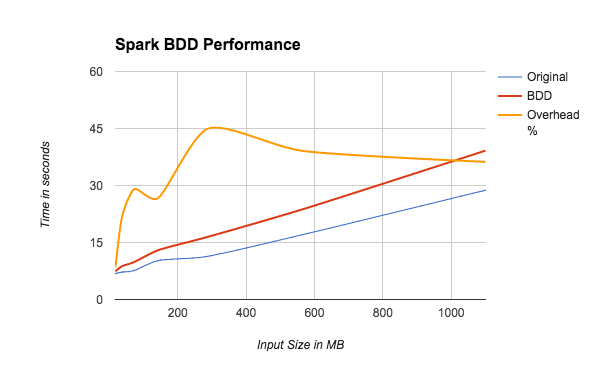
\includegraphics[width=\textwidth]{spark-bdd-performance.png}
        \caption{Overhead of Spark-BDD with all features enabled}
        \label{fig:overhead}
    \end{minipage}
\end{figure}
Our implementation of Spark-BDD poses 30\% of additional overhead with all debugging features enabled. The measurement on Spark-BDD is done by comparing total execution time between the original version of Spark and Spark-BDD. In Figure ~\ref{fig:overhead}, we can observe the relative percentage of overhead is not depending on the size of input data. Since we think superfluous information are easy to make a user confused, we set threshold of the maximum number of entries for each feature which has a proportional overhead on the data size.\\
\begin{figure}[ht]
    \begin{minipage}[b]{\linewidth}
        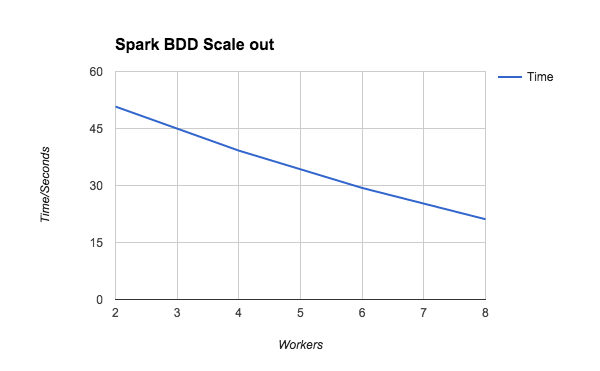
\includegraphics[width=\textwidth]{spark-bdd-scale-out.png}
        \caption{Scale-out of Spark-BDD}
        \label{fig:scaleout}
    \end{minipage}
\end{figure}
% Is the graph enough to rationalize the current implementation doesn't show any additional overhead as the number of workers increase. In my opinion, we need a dataset of the original version of Spark to evaluate the overhead properly.
% The large number of worker nodes doesn't guarantee the exact amount of performance boost.
Another possible factor of the overhead is the number of worker nodes. For example, the features of the breakpoint, watchpoint, straggler and re-partitioning can be affected by the number of worker nodes because it has to keep the status of each node. In Figure ~\ref{fig:scaleout}, we measured total execution time as the number of worker nodes increases. Considering the initialization time, performance overhead that is caused by the large number of worker nodes is negligible.

\section{Related work}
To our best knowledge, there are three systems designed for debugging cluster computing frameworks, Inspector Gadget~\cite{olston2011inspector}, Daphne~\cite{jagannath2011monitoring}, and Arthur~\cite{dave2013arthur}. 

Inspector Gadget is a framework for monitoring and debugging data flow programs in Apache Pig. It instruments programs to obtain various information, like the completion time of each task, records satisfying a predicate and report this information to developers. However, this approach requires the user to selectively specify the edges they want to monitor in the data flow graph, which we think is not very intuitive. Besides, the runtime overhead of IG sometimes jacks up to 70\%, which is very expensive in practice. In contrast, our approach allows users to debug data flow programs as they commonly do, by adding breakpoints and watchpoints and our approach only poses 30\% overhead. 

Daphne includes a set of tools that help developers visualize and debug DryadLINQ programs. Essentially, it models the distributed state of a program as a DryadLINQ job object. Layered on this model, they built various debugging features, e.g., collecting and analyzing performance data, visualizing distributed state, etc. This approach is limited because it requires the communication between tasks to be through files on disk. Thus, it is not applicable for frameworks that perform in-memory transformations such as Spark. However, Spark-BDD allows developers to view and reason about the intermediate data in Spark. 

Arthur provides a rich set of analysis tools through a selective replay of data flow applications in Hadoop and Spark. Instead of re-executing the entire program, it allows the user to selectively rerun the program to the point of interest. It further serializes the intermediate result at that point so the user can perform ad-hoc queries on the intermediate result. However, it has to replay the program from the beginning and doesn't allow the user to specify which dataset he or she wants to investigate. Spark-BDD overcomes these limits by allowing users to set breakpoints and watchpoints at any stage and any dataset as they wish.

\section{Conclusion}

\section{Future Work}
In the distributed computing system, faulty reasons can be from a lot of external sources. For example, a hardware failure, a link failure or the operating system level failure can crash the program. Thus, there is no guarantee that the crash culprits will reproduce the exactly same errors. To make sure the faults are coming from the value of a dataset, we are going to implement the feature of fault replay in local machines.\\
While a user develops Spark applications, the current version of Spark doesn't provide the visualization of the intermediate data summaries. We want to offer a clear view of data representation, therefore, the user can fix the program interactively.\\
Another future feature of our Spark-BDD is fault localization through forward and backward tracing.

\bibliographystyle{abbrv}
\bibliography{sigproc}  
\balancecolumns
% That's all folks!
\end{document}
